% !TeX root = ../../Book3.tex
% 纲要标题：### 18.4 曲面映射与复结构
% 纲要位置：几何学计划纲要.md，第 2852 行。
% 正文状态：初稿；尚未正式审核。

% 纲要内容开始
% 
% * 能量的共形不变性
% * Hopf 微分及全纯性
% * 共形调和映射与极小曲面
% * 气泡和同伦类丢失的模型
% 
% ---
% 
% 纲要内容结束

\section{曲面映射与复结构}
\label{g3:sec:1804}

在二维，把源度量放大时，微分的长度平方与面积元恰好按相反的比例变化。因此能量首先依赖曲面的共形结构，而不是某个指定的面积尺度。复坐标能把这种抵消写得很简洁，也能把调和方程中的一部分信息组织成全纯二次微分。另一方面，共形重参数化可以把整份能量压进越来越小的区域；本节末尾的球面模型将把这一现象逐项算出。
\ProseParagraphBreak
以下 \((\Sigma,g)\) 是光滑定向无边界二维黎曼流形，目标 \((N,h)\) 光滑且无边界，映射 \(u:\Sigma\to N\) 在讨论微分方程时均光滑。结论先在坐标区域中局部讨论，需要闭性时另行说明。沿用
\[
	e_g(u)=\frac12|\mathrm du|_{g,h}^2,\qquad
	E_g(u;\Omega)=\int_\Omega e_g(u)\,\mu_g,\qquad
	\tau_g(u)=\operatorname{tr}_g\nabla\mathrm du.
\]
其中 \(\Delta=-\operatorname{div}\operatorname{grad}\)，故 Euclid 目标时 \(\tau_g(u)=-\Delta_g u\)。

\subsection{能量的共形不变性}
\label{g3:subsec:1804:01}
\begin{proposition}\label{g3:prop:surface-energy-conformal}
	设 \((\Sigma,g)\) 为光滑无边界二维黎曼流形，\((N,h)\) 为光滑无边界黎曼流形，\(u:\Sigma\to N\) 光滑，\(\widehat g=e^{2\varphi}g\)，\(\varphi\in C^\infty(\Sigma;\mathbb R)\)。则
	\begin{equation}\label{g3:eq:surface-conformal-energy}
		e_{\widehat g}(u)=e^{-2\varphi}e_g(u),\qquad
		e_{\widehat g}(u)\mu_{\widehat g}=e_g(u)\mu_g,\qquad
		\tau_{\widehat g}(u)=e^{-2\varphi}\tau_g(u).
	\end{equation}
	因此任意区域上的能量相同，调和性也相同。若
	\(F:(\widetilde\Sigma,\widetilde g)\to(\Sigma,g)\) 是共形微分同胚，则
	\(E_{\widetilde g}(u\circ F;F^{-1}\Omega)=E_g(u;\Omega)\)。
\end{proposition}
\begin{proof}
	逆度量乘以 \(e^{-2\varphi}\)，二维面积密度乘以 \(e^{2\varphi}\)，前两个等式立即得到。为核对张力场，取任意紧支变分速度 \(V\)。两个能量作为变分的函数完全相同，\cref{g3:thm:harmonic-map-first-variation}于是给出
	\[
		\int_\Sigma\langle\tau_{\widehat g}(u),V\rangle
		e^{2\varphi}\mu_g
		=\int_\Sigma\langle\tau_g(u),V\rangle\mu_g.
	\]
	局部标架中的任意紧支测试截面均可实现为变分速度，故逐点有
	\(e^{2\varphi}\tau_{\widehat g}=\tau_g\)。最后把 \(F^*g\) 与
	\(\widetilde g\) 作上述比较，再使用积分换元公式。这里能量用密度积分，故重参数化是否保向不影响结论。
\end{proof}

一般实维数 \(m\) 时，相同计算给
\(e_{\widehat g}(u)\mu_{\widehat g}=e^{(m-2)\varphi}e_g(u)\mu_g\)。
二维的抵消因而是一项维数特征。要使用复变量，还需知道度量局部确实可以写成共形平面度量；这一步不能只由一个形式上的 \(90^\circ\) 旋转代替。

\begin{lemma}\label{g3:lem:surface-isothermal-coordinate}
	设 \((\Sigma,g)\) 为光滑定向无边界二维黎曼流形。每个点附近存在保向光滑坐标 \(z=x+iy\)，使
	\[
		g=\rho^2(\mathrm dx^2+\mathrm dy^2),\qquad \rho>0
	\]
	且 \(\rho\) 光滑。两张这样的保向坐标间的变换全纯、导数非零。因此它们确定一个只依赖 \(g\) 的共形类和定向的复图册。
\end{lemma}
\begin{proof}
	先构造一个梯度非零的局部调和函数，再以其调和共轭作第二个坐标。取中心为所给点的保向实坐标 \(\xi=(\xi^1,\xi^2)\)，经正行列式线性变换使 \(g_{ij}(0)=\delta_{ij}\)。在单位盘 \(B_1\subset\mathbb R^2\) 上设
	\[
		A_r^{ij}(y)=\sqrt{\det g(ry)}\,g^{ij}(ry).
	\]
	当 \(r>0\) 足够小时，这些矩阵一致正定，且
	\(\lVert A_r-I\rVert_{C^2(\overline B_1)}\le Cr\)。用\cref{g3:thm:weak-general-dirichlet}解
	\[
		-\partial_i(A_r^{ij}\partial_j h_r)=0
		\quad\text{于 }B_1,\qquad
		h_r=y^1\quad\text{于 }\partial B_1.
	\]
	这是实方程和实边值，唯一性保证解为实值。令 \(w_r=h_r-y^1\)，则
	\[
		-\partial_i(A_r^{ij}\partial_jw_r)=\partial_i A_r^{i1},
		\qquad w_r\in H_0^1(B_1).
	\]
	在弱方程中以 \(w_r\) 测试，并使用
	\(\int_{B_1}\partial_1w_r=0\)，得到
	\[
		c\lVert\nabla w_r\rVert_2^2
		\le \lVert A_r-I\rVert_\infty
		|B_1|^{1/2}\lVert\nabla w_r\rVert_2.
	\]
	\cref{g3:lem:boundary-poincare}的零边界估计给 \(\lVert w_r\rVert_{H^1}\le Cr\)。
	\cref{g3:thm:boundary-higher-regularity}中 \(k=1\) 的估计继而给出
	\[
		\lVert w_r\rVert_{H^3(B_1)}
		\le C\bigl(\lVert\partial_iA_r^{i1}\rVert_{H^1}
		+\lVert w_r\rVert_2\bigr)\le Cr.
	\]
	常数只依赖固定圆盘、统一椭圆下界及有限阶系数界，故可对小 \(r\) 统一选取。先用\cref{g3:prop:higher-order-boundary-extension}延拓，再用\cref{g3:cor:higher-sobolev-embedding}，所得二维 \(H^3\) 到 \(C^1\) 嵌入说明
	\(\mathrm dh_r(0)\to\mathrm dy^1\)。高阶正则性还给出 \(h_r\) 光滑。选定足够小的 \(r\)，把 \(h_r(\xi/r)\) 搬回原坐标，得到在中心附近满足 \(\Delta_g a=0\)、\(\mathrm da\ne0\) 的实函数 \(a\)。

	由\cref{g3:prop:codifferential-star}，二维一形式上
	\(\delta=-*\mathrm d*\)，所以 \(\mathrm d(*\mathrm da)=0\)。
	在中心为零的小坐标圆盘中，将闭一形式 \(*\mathrm da\) 写为
	\(\beta=\sum_j\beta_j(\xi)\mathrm d\xi^j\)，令
	\[
		b(\xi)=\int_0^1\sum_j\beta_j(t\xi)\xi^j\,\mathrm dt.
	\]
	闭性给出 \(\partial_k\beta_j=\partial_j\beta_k\)，故
	\[
		\partial_kb(\xi)
		=\int_0^1\frac{\mathrm d}{\mathrm dt}
		\bigl(t\beta_k(t\xi)\bigr)\,\mathrm dt=\beta_k(\xi).
	\]
	因此 \(\mathrm db=*\mathrm da\)。由星算子的定义，
	\[
		\langle\mathrm da,\mathrm db\rangle_{g^{-1}}=0,\qquad
		|\mathrm da|_{g^{-1}}=|\mathrm db|_{g^{-1}}>0,\qquad
		\mathrm da\wedge\mathrm db=|\mathrm da|^2\mu_g.
	\]
	故 \((a,b)\) 是保向坐标，其逆度量矩阵为
	\(|\mathrm da|^2I\)，即 \(g=|\mathrm da|^{-2}(\mathrm da^2+\mathrm db^2)\)。

	在两张此类坐标的交集上，变换的实微分是正比例伸缩与保向正交变换的复合。因此它满足 Cauchy--Riemann 方程；因变换光滑，这正是复可微性，逆变换也如此，故导数非零。最后，给 \(g\) 乘正函数不改变这组共形坐标，也就不改变所得复结构。
\end{proof}

这样的坐标称为\term[dengwen-zuobiao]{等温坐标}[isothermal coordinates]。在其中，任意光滑映射的局部能量变成
\begin{equation}\label{g3:eq:surface-energy-isothermal}
	E_g(u;\Omega)=\frac12\int_{z(\Omega)}
	\bigl(|u_x|_h^2+|u_y|_h^2\bigr)\,\mathrm dx\,\mathrm dy.
\end{equation}
这里 \(u_x=\mathrm du(\partial_x)\)、\(u_y=\mathrm du(\partial_y)\) 是沿 \(u\) 的向量，目标度量仍在 \(u(x,y)\) 处取值。消失的是源的共形因子，目标度量并没有被替换为常系数。

\subsection{Hopf 微分及全纯性}
\label{g3:subsec:1804:02}
在共形坐标中，能量使用 \(|u_x|^2+|u_y|^2\)，而是否保角还取决于两者是否等长、是否正交。把后两项组成一个复数，便得到
\[
	u_z=\frac12(u_x-iu_y),\qquad
	u_{\bar z}=\frac12(u_x+iu_y),\qquad
	q_u(z)=\langle u_z,u_z\rangle
	=\frac14\bigl(|u_x|^2-|u_y|^2-2i\langle u_x,u_y\rangle\bigr).
\]
此处目标度量在复化的拉回丛上作\emph{复双线性}延拓。若改用 Hermitian 延拓，\(\langle u_z,u_z\rangle\) 将成为非负长度平方，不能记录上述两个共形条件。

\begin{definition}\label{g3:def:hopf-differential}
	设 \((\Sigma,g)\) 为光滑定向无边界二维黎曼流形，\((N,h)\) 为光滑无边界黎曼流形，\(u:\Sigma\to N\) 光滑。其\term[Hopf-weifen]{Hopf 微分}[Hopf differential]在保向等温坐标中定义为
	\begin{equation}\label{g3:eq:hopf-differential}
		\Phi_u=\langle u_z,u_z\rangle\,\mathrm dz^2,
		\qquad \mathrm dz^2=\mathrm dz\otimes\mathrm dz.
	\end{equation}
	二次微分的局部系数在各张复坐标中全纯时，称它为全纯二次微分。
\end{definition}

这一定义与坐标选择无关。若 \(w=w(z)\) 是保向共形换坐标，则
\(u_w=u_z\,\mathrm dz/\mathrm dw\)，因此
\[
	q_{u,w}(w)=q_{u,z}(z)\left(\frac{\mathrm dz}{\mathrm dw}\right)^2.
\]
这恰是二次协变张量的变换律，且变换因子全纯、非零。第四卷第1.1.1小节中复可微与 Cauchy--Riemann 方程的等价，以及第2.1.1小节的复图册定义，与这里由度量构造的坐标完全相容。
% 跨卷依赖：g4:eq:0101:complex-linear；g4:def:0201:riemann-surface。

\begin{proposition}\label{g3:prop:hopf-holomorphic}
	设 \((\Sigma^2,g)\)、\((N,h)\) 为光滑无边界黎曼流形，\(\Sigma\) 定向，\(u:\Sigma\to N\) 光滑，\(g=\rho^2|\mathrm dz|^2\) 为保向等温坐标。以 \(D\) 表示拉回联络，令 \(D_{\bar z}=(D_x+iD_y)/2\)，则
	\begin{equation}\label{g3:eq:hopf-tension}
		D_{\bar z}u_z=\frac{\rho^2}{4}\tau_g(u),\qquad
		\partial_{\bar z}q_u
		=\frac{\rho^2}{2}\langle\tau_g(u),u_z\rangle.
	\end{equation}
	特别地，光滑调和映射的 Hopf 微分全纯。
\end{proposition}
\begin{proof}
	由\cref{g3:prop:map-covariant-identities}的无挠恒等式，
	\(D_yu_x=D_xu_y\)。于是
	\[
		D_{\bar z}u_z
		=\frac14(D_x+iD_y)(u_x-iu_y)
		=\frac14(D_xu_x+D_yu_y).
	\]
	对 \(g=\rho^2(\mathrm dx^2+\mathrm dy^2)\)，两个源联络项在取迹时相消：
	\(\nabla^g_{\partial_x}\partial_x+
	\nabla^g_{\partial_y}\partial_y=0\)。
	这可将共形度量的 Christoffel 公式直接代入核对，故
	\(\tau_g=\rho^{-2}(D_xu_x+D_yu_y)\)。第一式成立。目标联络保持度量，复双线性延拓后仍满足乘积法则，因而
	\[
		\partial_{\bar z}\langle u_z,u_z\rangle
		=2\langle D_{\bar z}u_z,u_z\rangle,
	\]
	得到第二式。若 \(\tau_g=0\)，则每张坐标中
	\(\partial_{\bar z}q_u=0\)，其光滑性使它全纯。
\end{proof}

全纯性并不意味着 \(\Phi_u=0\)。例如在标准平坦环面
\(\mathbb R^2/\mathbb Z^2\) 上，映射
\(u([x,y])=[2x,y]\) 到同一平坦环面是调和的，因为各局部分量的二阶导数为零；其 Hopf 微分却是
\(\frac34\,\mathrm dz^2\)。它沿两个方向的伸缩不同。

\begin{corollary}\label{g3:cor:harmonic-sphere-weak-conformal}
	设 \(S^2\) 带单位圆球度量与定向，\((N,h)\) 为任意光滑无边界黎曼流形。每个光滑调和映射 \(u:S^2\to N\) 都满足 \(\Phi_u=0\)。
\end{corollary}
\begin{proof}
	球面的复坐标为 \(z\in\mathbb C\) 与无穷远处的 \(w=1/z\)。若全纯二次微分在有限平面写作 \(q(z)\,\mathrm dz^2\)，则无穷远坐标中的系数为
	\(q(1/w)w^{-4}\)。它在 \(w=0\) 附近有界，故 \(q(z)=O(|z|^{-4})\)。
	因此 \(q\) 是有界整函数。第四卷第1.1.2小节的 Cauchy 估计给
	\(|q'(a)|\le \sup_{\mathbb C}|q|/R\)，对任意 \(R>0\) 成立。令 \(R\to\infty\)，得到 \(q'=0\)；再用无穷远处的衰减，得到 \(q=0\)。对 \(\Phi_u\) 应用上一命题即可。
	% 跨卷依赖：g4:prop:0101:cauchy-estimate；g4:subsec:0201:02。
\end{proof}

\subsection{共形调和映射与极小曲面}
\label{g3:subsec:1804:03}
光滑映射 \(u:(\Sigma,g)\to(N,h)\) 若满足
\[
	u^*h=\lambda^2g
\]
且 \(\lambda^2\) 是允许为零的非负函数，就称为\term[ruo-gongxing-yingshe]{弱共形映射}[weakly conformal map]。这里的“弱”表示允许微分退化；本段的映射本身仍是光滑的。在等温坐标中，这等价于
\(|u_x|=|u_y|\)、\(\langle u_x,u_y\rangle=0\)，也等价于 \(\Phi_u=0\)。
因此它在每一点的秩只能为 \(0\) 或 \(2\)，并且 \(\lambda^2=e_g(u)\)。
\ProseParagraphBreak
这个条件还可由面积与能量的比较辨认。对 \(g\) 正交归一基 \(e_1,e_2\)，设
\[
	J_2(u)=\sqrt{|\mathrm du(e_1)|^2|\mathrm du(e_2)|^2
	-\langle\mathrm du(e_1),\mathrm du(e_2)\rangle^2}.
\]
它是无符号的二维面积伸缩因子。若两个向量记为 \(a,b\)，则
\[
	e_g(u)^2-J_2(u)^2
	=\frac14(|a|^2-|b|^2)^2+\langle a,b\rangle^2\ge0.
\]
故参数面积 \(\operatorname{Area}(u;\Omega)=\int_\Omega J_2(u)\mu_g\) 不超过能量，逐点等号恰为弱共形条件。参数面积按覆盖重数计算，不能直接换成像集的面积。

\begin{proposition}\label{g3:prop:conformal-harmonic-minimal}
	设 \((\Sigma^2,g)\) 为光滑无边界二维黎曼流形，\((N,h)\) 为光滑无边界黎曼流形，
	\(u:\Sigma\to N\) 为光滑共形浸入，\(u^*h=\lambda^2g\)、\(\lambda>0\)。
	用诱导度量 \(\gamma=u^*h\) 定义第二基本形式 \(B^u\) 及平均曲率向量
	\(H^u=\frac12\operatorname{tr}_\gamma B^u\)。则
	\begin{equation}\label{g3:eq:conformal-tension-mean-curvature}
		\tau_g(u)=2\lambda^2H^u.
	\end{equation}
	因此 \(u\) 调和当且仅当 \(H^u=0\)，也即它是极小浸入。
\end{proposition}
\begin{proof}
	先把源赋予诱导度量 \(\gamma\)，此时 \(u\) 是等距浸入。
	\cref{g3:prop:gauss-decomposition}把
	\(D_X\mathrm du(Y)-\mathrm du(\nabla^\gamma_XY)\)
	识别为法向第二基本形式 \(B^u(X,Y)\)。取 \(\gamma\) 的迹，得
	\(\tau_\gamma(u)=2H^u\)。再由式\eqref{g3:eq:surface-conformal-energy}，
	\(\tau_\gamma=\lambda^{-2}\tau_g\)，即得所求等式。因 \(\lambda>0\)，两边的消失等价。平均曲率为零等价于紧支面积变分驻定，已由\cref{g3:cor:minimal-area-stationarity}证明。
\end{proof}

这里平均曲率取两个主方向的平均值，与第一卷第8.2.3小节的 \(H=(k_1+k_2)/2\) 一致；在任意余维中，它是法丛值向量，见\cref{g3:def:mean-curvature-vector}。对 Euclid 目标，式\eqref{g3:eq:conformal-tension-mean-curvature}也可写成
\(\Delta_g u=-2\lambda^2H^u\)，负号与本卷 Laplace 约定一致。
% 跨卷依赖：g1:def:surface-curvatures。
\ProseParagraphBreak
若 \(u\) 仅弱共形，结论首先适用于开集
\(\mathcal R=\{p:\mathrm du_p\ne0\}\)。在其补集上，诱导张量不是正定度量，不能在那里定义上述 \(H^u\) 后再除以 \(\lambda^2\)。对一个已经给定的光滑弱共形映射，若 \(\mathcal R\) 稠密且 \(H^u=0\) 于 \(\mathcal R\)，则连续性使 \(\tau_g=0\) 延续到全域；这项延续使用了映射跨越退化点的光滑性。
\ProseParagraphBreak
一个直接的分支模型是
\[
	u(z)=(\operatorname{Re}z^\ell,\operatorname{Im}z^\ell,0)
	\in\mathbb R^3,\qquad \ell\ge2.
\]
各分量调和，且 \(u^*h=\ell^2|z|^{2\ell-2}|\mathrm dz|^2\)。它在穿孔圆盘上共形浸入，在原点微分为零；这里的分支点及其有限阶来自显式幂模型。一般光滑弱共形调和映射的退化点是否孤立、是否有这样的有限阶表示，需要另外的局部理论，不由前一命题中的浸入公式推出。
\ProseParagraphBreak
特别地，曲面之间的保向共形局部微分同胚是调和的：目标与源同维，法丛为零，故 \(H^u=0\)。一个曲面之间的全纯映射也调和；在导数非零处用这条结论，在临界点用光滑性延续即可。确实，非恒定全纯函数的导数零点孤立，这是第四卷第1.1.3小节已经证明的幂级数零点性质；局部恒定情形本身也满足调和方程。反全纯映射的证明相同。
% 跨卷依赖：g4:thm:0101:identity；g4:thm:0101:local-power。

\subsection{气泡和同伦类丢失的模型}
\label{g3:subsec:1804:04}
把单位球面 \(S^2\subset\mathbb R^3\) 赋予圆球度量和外向定向。令
\begin{equation}\label{g3:eq:sphere-stereographic-parametrization}
	q(z)=\frac1{1+|z|^2}
	\bigl(2\operatorname{Re}z,-2\operatorname{Im}z,|z|^2-1\bigr),
	\qquad q(\infty)=p_+=(0,0,1).
\end{equation}
有限点坐标中的负号使 \(q\) 保向；在 \(z=0\) 处，其两个坐标切向量的叉积指向南极
\(p_-=q(0)=(0,0,-1)\)。直接微分得到
\[
	q^*g_{S^2}=\frac4{(1+|z|^2)^2}|\mathrm dz|^2.
\]
无穷远处使用 \(w=1/z\)，同样的表达光滑延拓。

\begin{example}\label{g3:exm:sphere-mobius-bubble}
	对 \(0<\varepsilon\le1\)，定义球面映射
	\[
		u_\varepsilon(q(z))=q(z/\varepsilon),
		\qquad u_\varepsilon(p_+)=p_+.
	\]
	这是光滑保向共形微分同胚，因而调和，且度数为 \(1\)。当
	\(\varepsilon\downarrow0\) 时，它满足
	\begin{align}
		E(u_\varepsilon)&=4\pi,\qquad
		u_\varepsilon\rightharpoonup p_+
		\quad\text{于 }H^1(S^2;\mathbb R^3),\label{g3:eq:sphere-bubble-weak-limit}\\
		e(u_\varepsilon)\mu_{S^2}
		&\rightharpoonup 4\pi\delta_{p_-}
		\quad\text{作为有限测度},\label{g3:eq:sphere-bubble-energy-measure}\\
		u_\varepsilon(q(\varepsilon w))&=q(w).\label{g3:eq:sphere-bubble-rescaling}
	\end{align}
	弱极限为度数 \(0\)、能量 \(0\) 的常值映射，且不存在向它强 \(H^1\) 收敛的子列。
\end{example}
\begin{proof}
	在有限坐标中，映射为 \(z\mapsto z/\varepsilon\)；在无穷远坐标中为 \(w\mapsto\varepsilon w\)。两处的复导数均非零，逆映射对应参数 \(1/\varepsilon\)，故它是保向共形微分同胚，调和性由上一小节得到。每个目标点恰有一个原像，且局部定向符号为正，所以度数为 \(1\)。也可用正参数的连续变化将它同伦到 \(u_1=\operatorname{id}\)。

	记 \(z=x+iy\)、\(r=|z|\)。目标拉回度量及能量测度为
	\begin{equation}\label{g3:eq:sphere-bubble-density}
		u_\varepsilon^*g_{S^2}
		=\frac{4\varepsilon^2}{(\varepsilon^2+r^2)^2}
		(\mathrm dx^2+\mathrm dy^2),\qquad
		e(u_\varepsilon)\mu_{S^2}
		=\frac{4\varepsilon^2}{(\varepsilon^2+r^2)^2}
		\,\mathrm dx\,\mathrm dy.
	\end{equation}
	第二式使用共形源中式\eqref{g3:eq:surface-energy-isothermal}的 \(1/2\) 归一化；两个正交方向给出相同贡献。极坐标积分给出
	\[
		E(u_\varepsilon)
		=8\pi\varepsilon^2\int_0^\infty
		\frac{r\,\mathrm dr}{(\varepsilon^2+r^2)^2}
		=4\pi.
	\]
	更准确地，若 \(D_R=\{q(z):|z|<R\}\)，则
	\begin{equation}\label{g3:eq:sphere-bubble-local-mass}
		E(u_\varepsilon;D_R)
		=4\pi\frac{R^2}{\varepsilon^2+R^2},\qquad
		E(u_\varepsilon;D_{\varepsilon R})
		=4\pi\frac{R^2}{1+R^2}.
	\end{equation}

	其外在表达为
	\[
		u_\varepsilon(q(z))
		=\frac1{\varepsilon^2+r^2}
		(2\varepsilon x,-2\varepsilon y,r^2-\varepsilon^2).
	\]
	对每个 \(z\ne0\)，此式趋于 \(p_+\)，在 \(p_+\) 处原本就是 \(p_+\)。
	所以除了单点 \(p_-\) 外处处收敛。映射值有界，球面体积有限，支配收敛给出
	\(u_\varepsilon\to p_+\) 于所有有限 \(L^p\) 空间。另一方面，
	\(\int_{S^2}|\mathrm du_\varepsilon|^2=8\pi\)，故这族在外在
	\(H^1(S^2;\mathbb R^3)\) 中有界。对任意光滑
	\(\phi:S^2\to\mathbb R^3\)，
	\[
		\int_{S^2}\langle\mathrm du_\varepsilon,\mathrm d\phi\rangle\mu
		=\int_{S^2}\langle u_\varepsilon,\Delta\phi\rangle\mu
		\longrightarrow
		\int_{S^2}\langle p_+,\Delta\phi\rangle\mu=0.
	\]
	光滑函数在 \(H^1\) 中稠密，再用统一梯度界，便得到整个族的弱
	\(H^1\) 收敛。若某子列强 \(H^1\) 收敛，强 \(L^2\) 极限只能是
	\(p_+\)，其梯度范数为零，却与恒等于 \(8\pi\) 的梯度范数平方矛盾。

	为证测度收敛，取任意 \(\psi\in C(S^2)\)，在能量积分中令
	\(z=\varepsilon w\)，得到
	\[
		\int_{S^2}\psi\,e(u_\varepsilon)\mu
		=\int_{\mathbb R^2}
		\psi(q(\varepsilon w))\frac4{(1+|w|^2)^2}
		\,\mathrm d(\operatorname{Re}w)\,\mathrm d(\operatorname{Im}w).
	\]
	权函数可积，总积分为 \(4\pi\)，被积函数逐点趋于
	\(\psi(p_-)\) 乘该权函数。支配收敛证明式\eqref{g3:eq:sphere-bubble-energy-measure}。最后直接代入定义，就得到式\eqref{g3:eq:sphere-bubble-rescaling}；重新放大后恢复的是整个非恒定球面参数映射。
\end{proof}

这个例子同时有两个观察尺度。固定 \(R>0\) 时，\(D_R\) 最终容纳几乎全部能量；固定放大坐标中的 \(R\) 时，\(D_{\varepsilon R}\) 所占比例始终为
\(R^2/(1+R^2)\)。令 \(R\to\infty\)，此比例趋于 \(1\)，所以该显式模型的全部 \(4\pi\) 能量都由重缩放后的球面恢复。
\begin{figure}[htbp]
	\centering
	% !TeX root = ../Book3.tex
\begin{tikzpicture}[x=3.1cm,y=3.7cm,>=stealth]
	\draw[->] (0,0)--(2.15,0) node[right] {\(R\)};
	\draw[->] (0,0)--(0,1.12) node[above] {\(E(u_\varepsilon;D_R)/(4\pi)\)};
	\draw[densely dotted,gray] (0,1)--(2,1);
	\node[left] at (0,1) {\(1\)};
	\draw[densely dotted,gray] (0,.5)--(1,.5);
	\node[left] at (0,.5) {\(\tfrac12\)};
	\draw[very thick,blue!75!black,domain=0:2,samples=101]
		plot (\x,{\x*\x/(.0625+\x*\x)});
	\draw[thick,red!75!black,dashed,domain=0:2,samples=101]
		plot (\x,{\x*\x/(1+\x*\x)});
	\draw[densely dotted,blue!75!black] (.25,0)--(.25,.5);
	\draw[densely dotted,red!75!black] (1,0)--(1,.5);
	\fill[blue!75!black] (.25,.5) circle (1.5pt);
	\fill[red!75!black] (1,.5) circle (1.5pt);
	\node[below] at (.25,0) {\(\tfrac14\)};
	\node[below] at (1,0) {\(1\)};
	\node[below] at (2,0) {\(2\)};
	\node[below left] at (0,0) {\(0\)};
	\draw[very thick,blue!75!black] (1.22,.35)--(1.4,.35);
	\node[right] at (1.42,.35) {\(\varepsilon=\tfrac14\)};
	\draw[thick,red!75!black,dashed] (1.22,.18)--(1.4,.18);
	\node[right] at (1.42,.18) {\(\varepsilon=1\)};
\end{tikzpicture}

	\caption[球面气泡的能量尺度]{圆盘内能量占总能量的比例为 \(R^2/(\varepsilon^2+R^2)\)。当 \(R=\varepsilon\) 时恰好容纳一半能量；\(\varepsilon\) 越小，同一份能量进入越小的坐标圆盘。}
	\label{g3:fig:bubble-energy-scale}
\end{figure}

为了在后面的具体例子中计算总能量，也可用度数。若
\(v:\Sigma\to S^2\) 是闭连通定向曲面上的光滑映射，记圆球的定向面积形式为 \(\omega\)，令 \(v^*\omega=j_v\mu_g\)。逐点有
\[
	|j_v|\le e_g(v).
\]
第二卷第16.1.2小节的度数与积分比较公式给出
\[
	\int_\Sigma j_v\mu_g=4\pi\deg v,\qquad
	E_g(v)\ge4\pi|\deg v|.
\]
这里光滑性、闭性和两边相同的实维数正是度数积分公式的假设。保向弱共形映射满足 \(j_v=e_g(v)\)，所以其能量恰为 \(4\pi\deg v\)；反向情形相应取负号。这个计算也说明上面的 \(4\pi\) 来自一次覆盖球面的面积。
% 跨卷依赖：g2:thm:degree-comparison；g2:eq:degree-integral。
\ProseParagraphBreak
在弱极限中丢失的不是“取值仍在球面”这一条件。由于
\(u_\varepsilon\to p_+\) 强 \(L^2\)，且球面是闭集，极限依然取值于球面，符合前面 Sobolev 映射的闭目标约束。丢失的是度数所区别的同伦类以及梯度的强收敛：每个 \(u_\varepsilon\) 的度数为 \(1\)，常值极限的度数为 \(0\)，而能量留在集中点的测度中。这里的调和方程在极限下仍成立，因为常值映射调和；因此“极限仍调和”和“同伦类、能量都被保留”是不同的结论。
% 纲要条目排为编号小节标题，并进入目录与书签；说明段仍保留于纲要注释中。
